\chapter{Results}%
\label{chap:results}
\textit{This chapter presents the test results that test and challenge the proposed method. Three types of test are introduced which are custom made benchmark tests, randomization tests and test taken including and excluding the \ac{kgraph}. The test results provide evidence that support the effectiveness of the proposed method. This chapter starts by introducing \textbf{method metrics} that indicate how a task has been executed by the proposed method in \Cref{sec:proposed_method_metrics}. Then the three types of test are presented in \Cref{sec:benchmark_tests,sec:randomisation,sec:kgraph_on_off}. A comparison is made with the state-of-the-art methods in \Cref{sec:compare_with_related_papers}, the chapter is finalized with a discussion about the results in \Cref{sec:discussion}.\bs}
\todo[inline]{update intro above}

\paragraph{The Simulation Environment}
Testing in a simulation environment has been done using the URDF Gym Environment~\cite{spahn_urdfenvironment_2022}, a 100\% python environment build upon the PyBullet library~\cite{coumans_pybullet_2016}. The code created during the thesis can be found on \href{https://gitlab.tudelft.nl/airlab-delft/msc_projects/msc_gijs_groote}{GitLab} and \href{https://github.com/GijsGroote/semantic-thinking-robot}{GitHub}. Experiments ran on standard TU Delft laptop: HP ZBook Studio x360 G5, running OS:~Ubuntu 22.04.1 LTS x86\_64, CPU: Intel i7-8750H (12) @ 4.100GHz, GPU: NVIDIA Quadro P1000 Mobile.\bs
The simulation environment provides many different robots, 2 simple robots are selected to perform tests, they are displayed in \Cref{fig:example_robots}, and various objects are displayed in \Cref{fig:example_objects}.

\section{Proposed Method Metrics}%
\label{sec:proposed_method_metrics}
The results are measured in method metrics, not to be confused with the monitoring metrics in \Cref{sec:monitoring_metrics} or the edge metrics in \Cref{subsec:edge_metrics}. The results are interesting, but most interesting is the progression of the method metrics over time. As will be shown, the effect of learning can be measured by investigating tracking the method metrics over time. Furthermore, the method metrics will be used to compare the proposed method to relative state-of-the-art papers. First the method metrics are presented in~\Cref{table:proposed_method_metrics} with corresponding argumentation on the relevance of the metric.\bs

\noindent
\begin{table}[H]
\centering
\begin{tabular}%
  {>{\raggedright\arraybackslash}p{0.25\textwidth}%
   >{\raggedright\arraybackslash}p{0.65\textwidth}}
Total Average\newline \acl{PE} & The total average \ac{PE} is created by averaging over every hypothesis' average \ac{PE} in a \ac{hgraph}. Since the \ac{PE} is high when unexpected behavior occurs, seeing the total average \ac{PE} lower would indicate the robot encounters less unexpected behavior, indicating the robot is learning.\\
Total Average\newline \acl{TE}& The total average \ac{TE} is created by averaging over every hypothesis' average \ac{TE} in a \ac{hgraph}. Seeing the total average \ac{TE} lower over time would indicate the robot is selecting better suitable controllers and system models, indicating the robot is learning.\\
Final positions and\newline displacement errors & The final position and displacement error is a metric which how a controller performs. This thesis does not create or investigate controllers, but it is interesting to see why different controllers are preferred for different objects. The final position and displacement error could be the cause.\\
The ratio between the number of hypothesis and the number of tasks & Expected is that whilst learning system models, the hypothesis created will be more effective. Thus the ratio between the total number of hypotheses and the total number of tasks is expected to lower with new knowledge.\\
The ratio between the number of successful and the number of total edges in \ac{kgraph} & When the \ac{kgraph} improves recommending a controller and system model, the ratio between successful edges and total edges is expected to increase because, with better recommendations, more edges will be successfully completed.\\
task completion time =\newline run time + planning time& If equal tasks are given multiple times, the total task completion time should drop pretty drastically. Multiple factors help to lower the task completion time, firstly system identification has to be performed only once, and there is no need to lose time on redoing system identification. Secondly, the \ac{hgraph} is expected to improve generated hypothesis, or better said, the same mistake should not be made multiple times, resulting in fewer failing hypotheses and lowering task completion time.\\
\end{tabular}
\caption{Proposed method metrics used to compare the proposed method with the state-of-the-art methods.}\label{table:proposed_method_metrics}
\end{table}


\todo[inline]{define nonlinear-drive-model}
\todo[inline]{define lti-drive-model}
\todo[inline]{define nonlinear-push-model-2}
\todo[inline]{define nonlinear-push-model-2}

% \section{Benchmark Tests}%
% \label{sec:benchmark_tests}
% Three benchmark test are presented, starting with the blockade task. A large part of the proposed method is system identification, for testing however no system identification is performed. Instead a number of hard coded system models are used, the \ac{kgraph} finds which system model is the best choice for an object over time. Where the best choice is defined using the edge metrics discussed in \Cref{subsec:edge_metrics}. The hard coded system models are not opting for modeling the drive or push model as accurate as they possibly can, thus severe model mismatch should be expected. Such model mismatch is no issue, to complete a subtask stable closed-loop control is required, when an edge parameterization is unable so provide closed-loop stable control, the edge will fail because an fault will be detected. To answer the research question, improvement over time should be made. Gaining such improvement does not require accurate system models, time spend improving the hand coded system models does thus not change the result.\bs
%
%
% \paragraph{Blockade} In the blockade environment the robot is tasked with placing a box to a target position that is blocked by an cylinder object.\bs
% \begin{figure}[H]
%     \centering
%     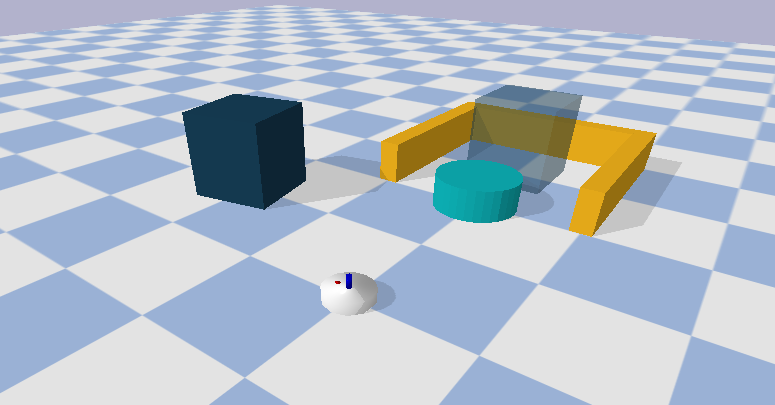
\includegraphics[width=0.9\textwidth]{figures/tests/blockade}
%     \caption{The blockade environment with the target ghost position for the blue box. The green walls are unmovable whilst both the blue box and cylinder are movable.}%
%     \label{fig:benchmark_blockade}
% \end{figure}
%
% The blockade task neatly shows that the \ac{halgorithm} uses the backward search technique. First the \ac{halgorithm} plans to push the box directly to the target position, then it realizes a blocking object must first be moved to free the path. It makes the mistake of pushing the unmovable wall, then it succeeds in pushes the movable cylinder out of the way. The \ac{kgraph} then ensures that this mistake will not occur again because is remembered that the wall is immovable. Over time the \ac{kgraph} indicates that it prefers to use the \ac{MPPI} controller with the nonlinear-push-model-2 to push both the box and the cylinder object. Converging to this conclusion improves the method metrics for the task as can be seen in \Cref{fig:results_blockade}\bs
%
% \todo[inline]{is nonlinear-push-model-2 still the preferred model after testing??}
%
% \begin{figure}[H]
%     \centering
%     
\includegraphics[width=0.9\textwidth]{figures/tests/404_not_found}
%
%     \caption{Some test are still under development for the blockade environment}%
%     \label{fig:results_blockade}
% \end{figure}
% \todo[inline]{Test to create results for running the blockade environment, and input into above 404 not found}
%
% \paragraph{Swap}
% In the swap environment the robot should swap the locations of the 2 objects in the environment.\bs
%
% \begin{figure}[H]
%     \centering
%     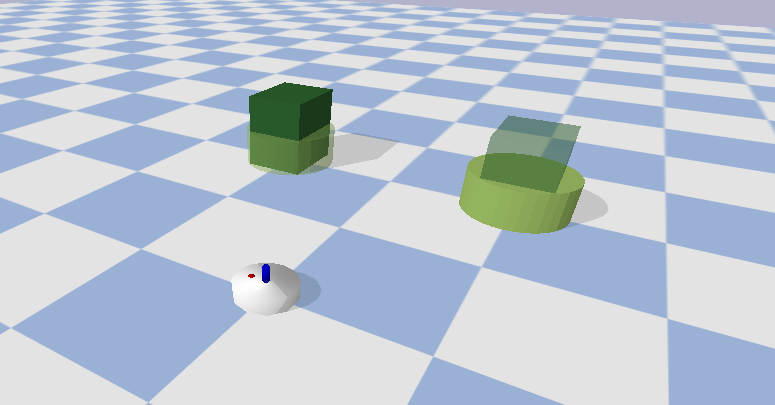
\includegraphics[width=0.9\textwidth]{figures/tests/swap}
%     \caption{The swap environment, the robot is tasked with swapping the positions of the cylinder and the box.}%
%     \label{fig:benchmark_swap}
% \end{figure}
% The swap task shows that the \ac{halgorithm} can handle overlapping subtasks. The \ac{halgorithm} handles a single subtask at a time and randomly selects which subtask to handle next. The result for the swap task is that, first the robot will place the box on the location of the cylinder. The cylinder is blocking the path and is thus pushed to free the path, then the robot drive back to the box to push the box to its target position. The cylinder can directly be pushed toward its target position, because there is a free path, and the task is successfully completed. By manual inspection, this is the most efficient action sequence to complete the swap task. But there is an assumption, because the initial environment has a distance between the robot and box (robot-box distance), and robot and cylinder (robot-cylinder distance) that is equal. If the initial robot-box distance is greater than the initial robot-cylinder distance, it would be more efficient to first drive toward the cylinder because that distance is smaller. The selection of subtask is at random, thus there is a 50\% chance that the robot selects a subtask resulting in driving more than is necessary to complete the swap subtask.\bs
%
% \begin{figure}[H]
%     \centering
%     
\includegraphics[width=0.9\textwidth]{figures/tests/404_not_found}
%     \caption{Some test are still under development for the swap environment}%
%     \label{fig:results_swap}
% \end{figure}
%
% \todo[inline]{Test to create results for running the swap environment}
%
% \paragraph{Surrounded} In the surround environment the robot has to learn which box is movable to escape the enclosure of boxes.\bs
% \begin{figure}[H]
%     \centering
%     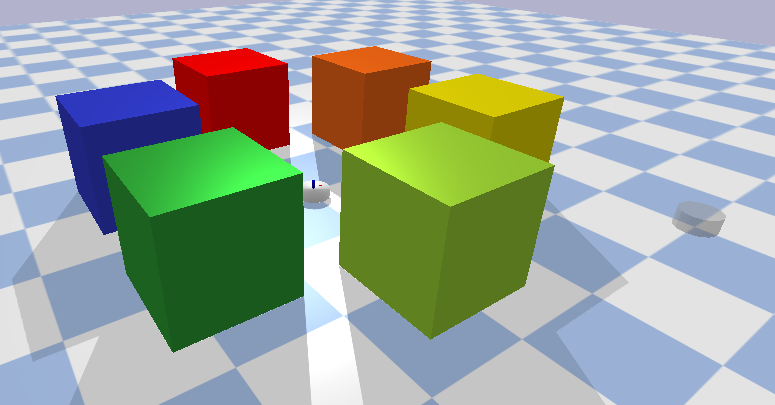
\includegraphics[width=0.9\textwidth]{figures/tests/surrounded}
%     \caption{The surround environment, the robot is tasked with escaping the surrounding enclosure by driving to the target ghost position displayed on the right side in the figure. Every box objects is unmovable except the red box which is movable.}%
%     \label{fig:benchmark_surround}
% \end{figure}
% The surround task show that having and gaining environment knowledge can greatly improve task execution. Simply knowing if an object can be interacted with may lower task execution time drastically as can be seen in \Cref{fig:results_surround}.\bs
%
% \begin{figure}[H]
%     \centering
%     
\includegraphics[width=0.9\textwidth]{figures/tests/404_not_found}
%     \caption{Some test are still under development for the surround environment}%
%     \label{fig:results_surround}
% \end{figure}
%
% \todo[inline]{Test to create results for running the surround environment}

\section{Randomization}%
\label{sec:randomisation}
In the randomized environment the robot is tasked to push a number of object to a target location. The previous 3 benchmark tests are designed around the proposed method, meaning that these test highlight the strong points of the \ac{halgorithm} but prevent the testing the weak points of the proposed methods. Such bias can lead to false positives, which is undesired. The randomized environment provides an more unbiased results. The random environment does not deliver completely unbiased results because there are several parameters that must be chosen to create and set up the random environment, which are.\\

\noindent
\begin{table}[H]
\centering
\begin{tabular}%
{>{\raggedright\arraybackslash}p{0.25\textwidth}%
>{\raggedright\arraybackslash}p{0.65\textwidth}}
The \textit{size of the grid} & in \gls{x} and \gls{y} direction.\\
The \textit{minimal and maximal size of objects} & A box will have sides with length that lie in the specified range from minimal to maximal length. Cylinders will have a diameter and height that is between the specified range, additionally cylinders are not higher than the radius of the cylinder to prevent cylinders tipping over. \\
The \textit{maximal weight} & which is uniformly distributed for the environment objects, minimal weight is set by default to 0. \\
The \textit{number of unmovable and movable objects} & For every new object generated there is a 50\% chance it becomes a box and 50\% chance it becomes a cylinder, letting randomization determine the ratio between boxes and cylinders. \\
The \textit{number of subtasks in a task} & Which must be greater or equal to the number of movable objects. The task has feasible targets that lie in free space, the path estimator discussed in \Cref{subsec:path_estimation} is used to determine the target configuration for objects. By creating configuration space for an object the target configuration is chosen to be in free space, then path estimation is used to determine if an object can reach the target configuration from its initial configuration.
\end{tabular}
\end{table}

If the task is completed, a \textit{reshuffle} function reshuffles the objects in the environment, that is the object remain the same objects, but the objects receive a new initial position, and the subtask target configurations are renewed. The reshuffled environments can be seen in \Cref{fig:random_environment_reshuffle}.\bs

\begin{figure}[H]
    \centering
    \begin{subfigure}{\textwidth}
    \centering
    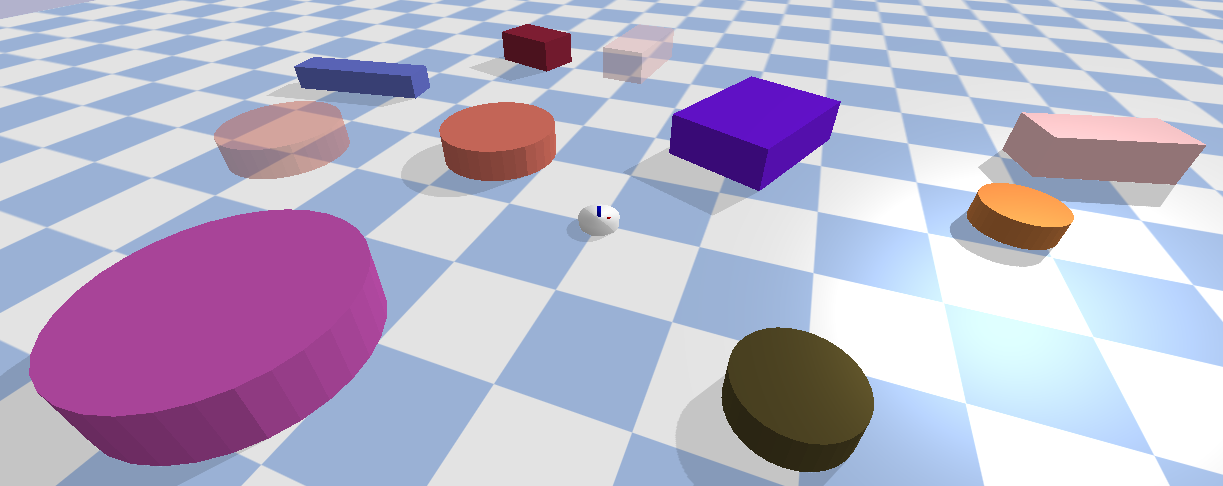
\includegraphics[width=0.9\textwidth]{figures/tests/random_1}
    \end{subfigure}

    \vspace{0.2cm}
    \begin{subfigure}{\textwidth}
    \centering
    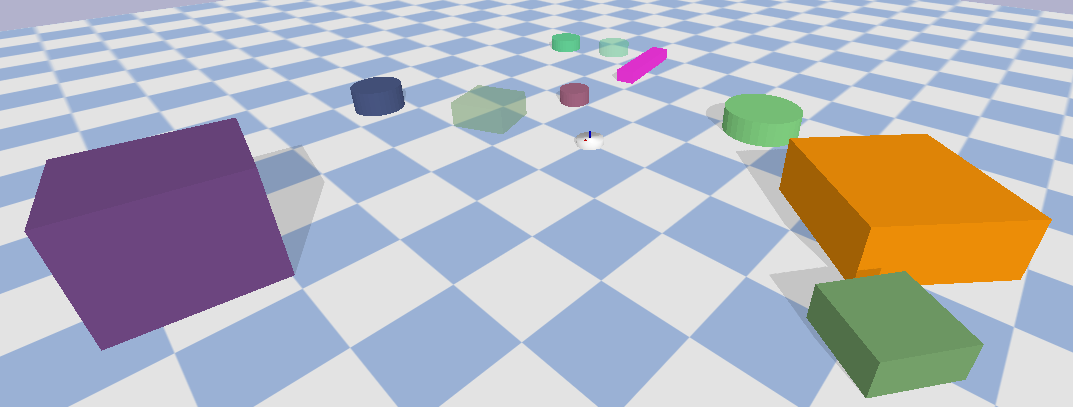
\includegraphics[width=0.9\textwidth]{figures/tests/random_2}
    \end{subfigure}
    \caption{Two random environment with 2 target ghost configurations for the task containing 2 subtasks.}%
    \label{fig:random_environnment}
\end{figure}

\begin{figure}[H]
    \centering
    \begin{subfigure}{.49\textwidth}
    \centering
    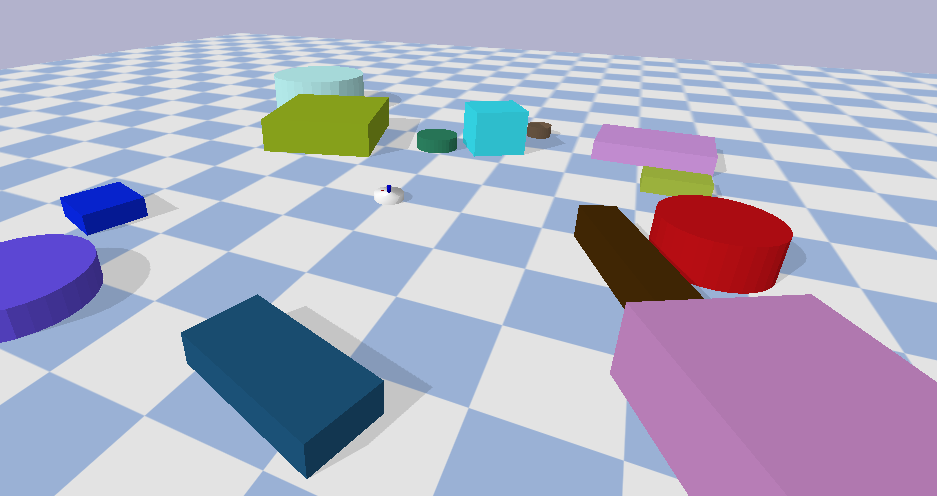
\includegraphics[width=\textwidth]{figures/tests/random1}
    \end{subfigure}
    \hfill
    \begin{subfigure}{.49\textwidth}
    \centering
    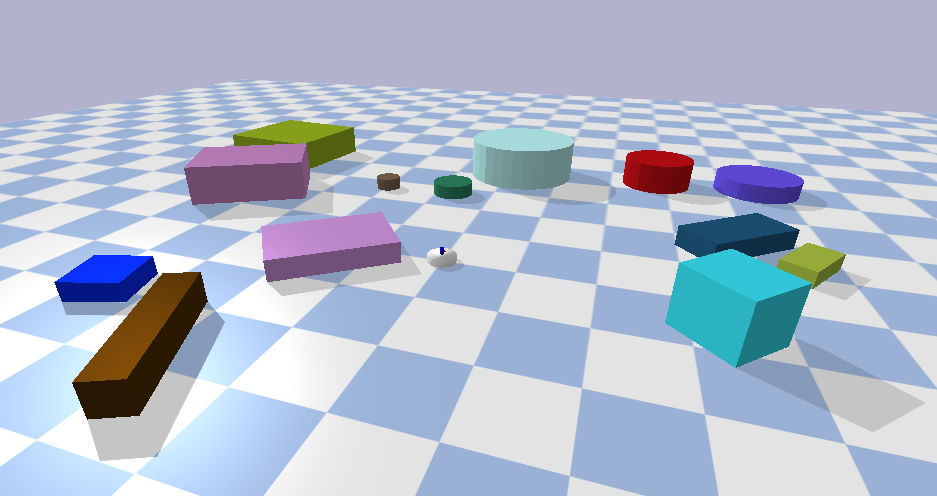
\includegraphics[width=\textwidth]{figures/tests/random2}
    \end{subfigure}

    \vspace{0.2cm}
    \begin{subfigure}{.49\textwidth}
    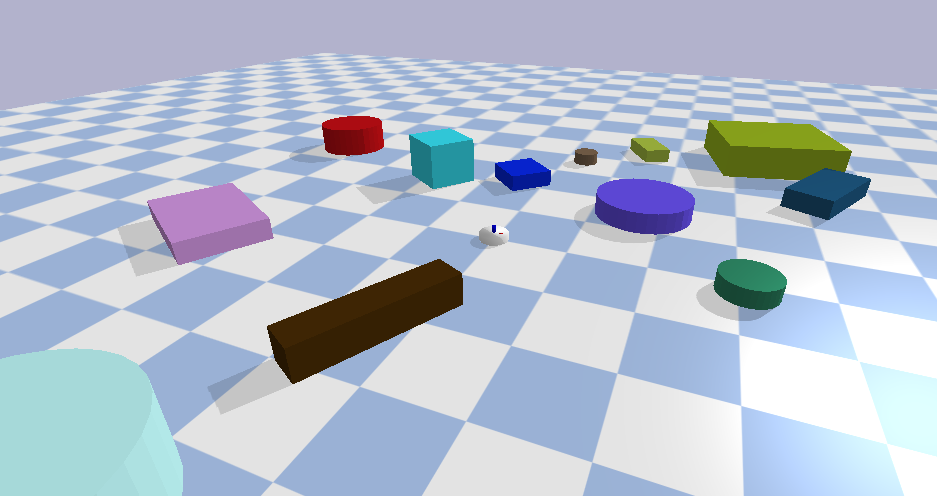
\includegraphics[width=\textwidth]{figures/tests/random3}
    \end{subfigure}
    \hfill
    \begin{subfigure}{.49\textwidth}
    \centering
    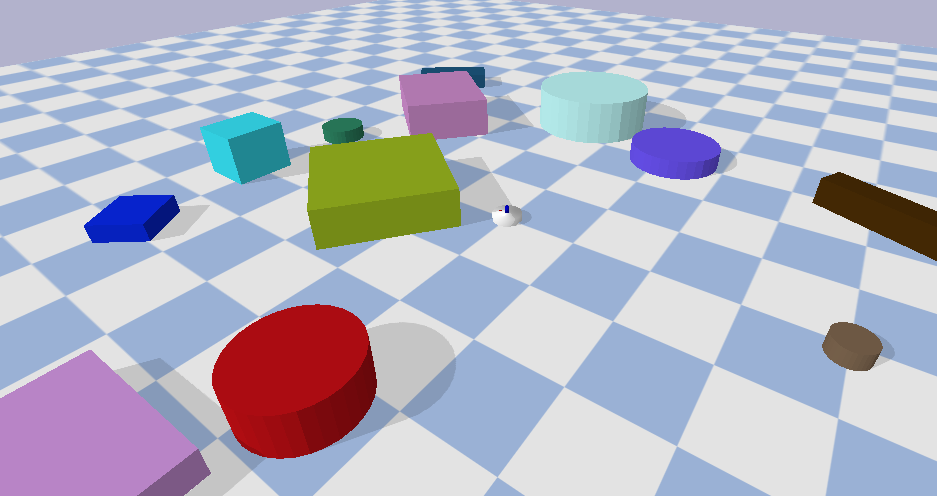
\includegraphics[width=\textwidth]{figures/tests/random4}
    \end{subfigure}
    \caption{A random environments that is reshuffled 4 times. Target ghost configurations are not shown.}
    \label{fig:random_environment_reshuffle}
\end{figure}

The \ac{halgorithm} will be tested with both driving and pushing tasks. Starting with driving tasks for which the parameters are set to be.\bs

\begin{center}
\begin{align*}
\text{grid size} \quad &\gls{x}=12, \quad \gls{y}=12 \\
\text{object size} \quad &\mathit{min\_length}=0.2, \quad \mathit{max\_length}=2 \\
\text{object weight} \quad &\mathit{max\_weight}=1000 \\
\text{number of objects} \quad &\mathit{num\_unmovable\_obj}=3, \quad \mathit{num\_movable\_obj}=5 \\
\text{number of subtasks} \quad &\mathit{num\_subtasks}=3
\end{align*}
\end{center}

These parameters have been specifically selected, starting with the size of the ground floor. The ground floor should be large enough such that objects can be pushed around, note that, for a driving task, pushing is involved when a path must be freed. Environments must thus not be to small. A ground floor too large would result in a longer computational time for path estimation and planning which is undesired. A 12 by 12 is selected because it is reflecting a reasonably large workspace, whilst computation times for planning are kept at similar to computation times. The range that determines the size of objects is set such that objects can be as large as the robot itself, and be around 10 times as large as the robot. With these sized the robot is unable to grasp objects, a gripper would be to small to grasp objects. The comparatively large size fits the objective of nonprehensile pushing, there simply is not other method to manipulate such large objects other then pushing. A real life example are can be found in harbors where tug boats push giant cargo ships around that are many times over the size of the tug boat. The ratio of solid obstacles vs.~movable objects determine if a task is more navigation (only solid obstacles) or more \ac{NAMO} (only movable objects). A task that tends toward \ac{NAMO} is favored because that is the target environment int this thesis. There should be some unmovable obstacles that reward the robot learning such objects are unmovable (to then not interact with them). Thus there are more movable objects than solid obstacles chosen, whilst still having 2 solid obstacles around. The number of subtasks is set to 3, a low number of drive subtasks that can be completed in under 2 minutes.\bs


The following figure shows a driving task containing 3 subtasks for the robot. The randomly generated task in the random environment is reshuffled and then solved 10 times. The sequence of tasks is performed once with the \ac{kgraph} suggestions. Then the same environments and tasks are solved 10 times without the \ac{kgraph} suggestions. The randomly generated tasks and environments are repeatable by fixing the seed. The fixed seed ensures that the randomly generated environments for solving tasks with \ac{kgraph} is equal to the environments for solving tasks without the \ac{kgraph}.\bs

\begin{figure}[H]
    \centering
    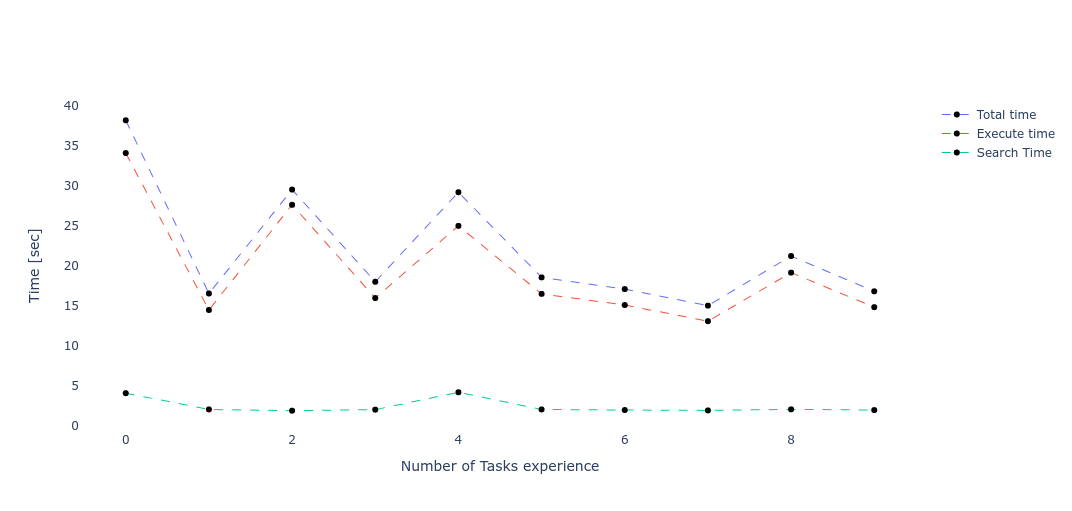
\includegraphics[width=0.9\textwidth]{figures/results/random_drive_execution_times}
    \caption{Execution times for driving toward target configurations with and without \ac{kgraph}.}%
    \label{fig:results_random_drive_task}
\end{figure}

The figure above shows similar running times at the first few solved tasks. During these first tasks the \ac{kgraph} is filled with edge feedback, but the \ac{kgraph} has not gained enough feedback to suggest action parameterizations this period can be referred to as the learning phase. After this learning phase, the \ac{kgraph} suggests the \ac{MPC} controller with its corresponding system model, because of its higher \textit{success factor} compared to the \ac{MPPI} controller. The action suggestions improve overall execution time, note that selecting random controllers can result in equal execution time. In these cases, (4, 7 or 9 tasks in experience in \cref{fig:results_random_drive_task}) the randomly selected controllers all were \ac{MPC} controllers.\bs

Now the \ac{halgorithm} is tasked with pushing a single object toward a target configuration. Once again with the \ac{kgraph} action suggestions and once without action suggestions. Except for the number of subtasks all parameters that determine the random environment will remain as previously set for the random driving task.\bs

\begin{figure}[H]
    \centering
    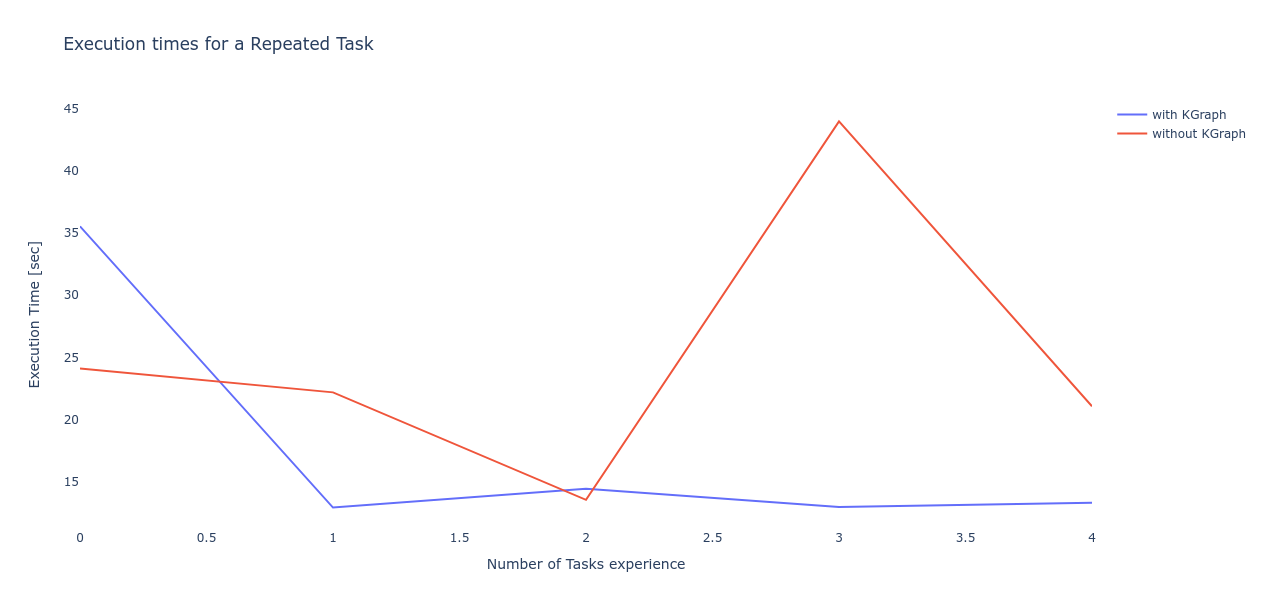
\includegraphics[width=0.9\textwidth]{figures/results/random_push_execution_times}
    \caption{Planning times for driving toward target configurations with and without \ac{kgraph}.}%
    \label{fig:random_push_with_without_kgraph}
\end{figure}

Initially the randomly selected controller had a lower execution time compared to solving the same task with \ac{kgraph}. After a single task of experience, the \ac{halgorithm} with \ac{kgraph} prefers to use the \ac{MPPI} controller with nonlinear model 2. Resulting in solving a pushing task in under 15 seconds of execution time. 

% \section{Knowledge Graph On/Off}%
% \label{sec:kgraph_on_off}
% Influence of the \ac{kgraph} is shown using the random environment. The robot will once complete many random tasks with the help of \ac{kgraph} and once the robot will complete many random tasks without the help of \ac{kgraph}. The results can be compared in \Cref{fig:results_random_kgraph_on_off}.\bs
%
% \begin{figure}[H]
%     \centering
%     
\includegraphics[width=0.9\textwidth]{figures/tests/404_not_found}
%     \caption{Some test are still under development for the randomization where the kgraph is once on and once off.}%
%     \label{fig:results_random_kgraph_on_off}
% \end{figure}
%
% \todo[inline]{Test to create results for running (run that many times) the random environment}
%

\section{Comparison with State-of-the-Art}%
\label{sec:compare_with_related_papers}

The papers to compare with:\newline

\citefield{sabbaghnovin_model_2021}{title}\\

\cite{sabbaghnovin_model_2021},
\todo[inline]{See the paper for tests to reproduce with my hgraph}


\citefield{novin_dynamic_2018}{title}\\
\cite{novin_dynamic_2018}
The following \cite{novin_dynamic_2018} citation is here because it is a referred to from~\cite{sabbaghnovin_model_2021} many times




\section{Discussion}%
\label{sec:discussion}
